\documentclass[a4paper]{article}
\usepackage{polyglossia}
\setmainlanguage{spanish}
\setmainfont{Carlito}
\usepackage{anyfontsize}
\usepackage{fontspec}
\usepackage{setspace}
\singlespacing
\usepackage{textcomp,marvosym,pifont}
\usepackage[a4paper,top=3cm,bottom=2cm,left=3cm,right=3cm,marginparwidth=1.75cm]{geometry}
\usepackage{amsmath, amsthm, amsfonts}
\usepackage{graphicx}
\usepackage[colorlinks=true, allcolors=blue]{hyperref}
\setlength{\parskip}{1.5mm}

\title{Inferencia verificable en modelos de Aprendizaje Automático mediante Pruebas de Conocimiento
Cero}
\author{Álvaro Martínez Alfaro\\
  \small alvaro.martinez39@alu.uclm.es\\
  \small Criptografía, ESII, Universidad de Castilla-La Mancha\\
  \small Albacete, España
}

% ==================================================================================================

\begin{document}

\maketitle

%% Resumen
\begin{abstract}
  % TODO: escribir resumen.

\end{abstract}

% Introducción
\section{Introducción}


% Fundamentos teóricos
\section{Fundamentos teóricos}
En esta sección se presentan los conceptos teóricos necesarios para el desarrollo del trabajo,
incluyendo una introducción a los modelos de aprendizaje automático, las pruebas de conocimiento
cero y los fundamentos matemáticos sobre los que se asientan.

\subsection{Aprendizaje Automático}
El \textbf{aprendizaje automático} es una rama de la inteligencia artificial centrada en conseguir
que los ordenadores simulen la capacidad humana de \textit{aprender}, así como de buscar métodos que
les permitan adquirir conocimientos y habilidades para mejorar su rendimiento ante determinadas
tareas \cite{5362936}. A diferencia del aprendizaje humano, que se construye a base de la
experiencia adquirida a lo largo de grandes períodos de tiempo, los sistemas de aprendizaje
automático, gracias a la potencia de cálculo de los ordenadores, pueden adquirir conocimientos
utilizando grandes cantidades de datos en períodos de tiempo relativamente cortos; apenas unos
minutos en modelos simples y con conjuntos de datos pequeños, como sería el caso de un
\textit{árbol de decisión}, u horas, días o incluso semanas en modelos complejos y con conjuntos de
datos masivos, como es el caso de los \textit{grandes modelos de lenguaje}.

\subsubsection{Redes neuronales artificiales}

Si hay un modelo de aprendizaje automático que ha adquirido notoriedad en las últimas décadas, ese
es el de las \textbf{redes neuronales artificiales}, incluyendo todas sus variantes. Desde una
perspectiva biológica simplificada, el cerebro humano se compone de una gran cantidad de
\textit{neuronas} interconectadas entre sí que se comunican mediante \textit{impulsos eléctricos}
que reciben a través de sus \textit{dendritas} y transmiten a través de sus \textit{axones}
\cite{article}. De manera similar, las redes neuronales artificiales se componen de unidades
denominadas \textit{neuronas artificiales}, conectadas entre sí mediante \textit{enlaces} que
transmiten señales. Concretamente, estas señales se representan mediante \textit{números reales},
donde cada uno de ellos simboliza la fuerza de la conexión, también conocida como \textit{peso}. Una
red neuronal suele contener desde algunas decenas hasta miles o incluso millones de neuronas
artificiales, organizadas en diferentes \textit{capas}. Las neuronas de cada capa se encuentran
conectadas a las de la capa siguiente. Un ejemplo típico de red neuronal se muestra en la Figura
\ref{fig:nn}, la cual está compuesta por una capa de entrada, dos capas ocultas y una capa de
salida. Cuando una red neuronal contiene una o más capas ocultas, se denomina
\textit{red neuronal profunda}, siendo este el caso mostrado y, en general, el más común en la
actualidad.

\begin{figure}
  \centering
  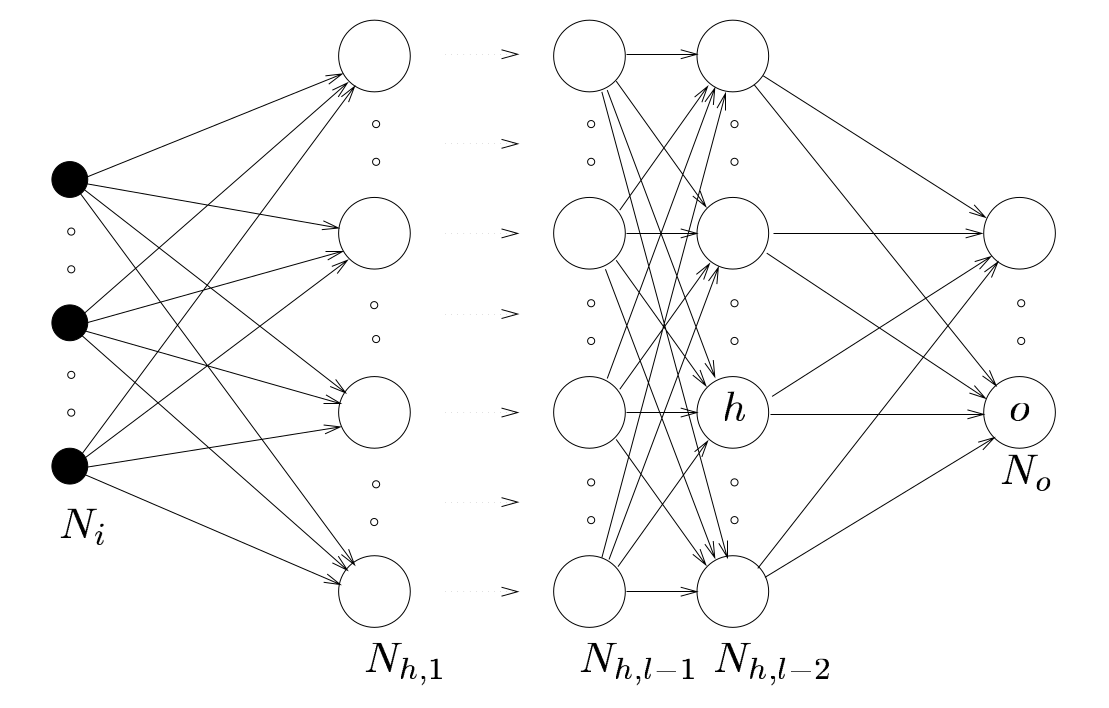
\includegraphics[width=0.6\textwidth]{figs/nn.png}
  \caption{Ejemplo de red neuronal artificial.}
  \label{fig:nn}
\end{figure}

En cada neurona, se realiza una suma ponderada de las señales recibidas a través de sus enlaces, de
forma que, en una cierta neurona $k$, la entrada total que recibe en un instante de tiempo $t$ viene
dada por
\begin{equation}
  s_k(t) = \sum_{j} w_{jk}(t) y_j(t) + \theta_k(t) \label{na_entrada_total}
\end{equation}
donde $w_{jk}(t)$ representa el peso del enlace que conecta la neurona $j$ con la neurona $k$,
siendo $j$, normalmente, una neurona de la capa anterior \cite{krose1996introduction}. Cuando el
peso es positivo, se dice que el enlace es \textit{excitatorio}, mientras que, si es negativo, se
dice que es \textit{inhibitorio}. Luego, $y_j(t)$ representa la señal de salida de la neurona $j$ y,
finalmente, $\theta_k(t)$ representa el \textit{sesgo} de la neurona $k$, un valor constante que
permite ajustar su umbral de activación.

Tras ello, la neurona $k$ aplica una \textit{función de activación} a su entrada total, $s_k(t)$,
para generar su salida $y_k(t+1)$. Así, la salida de la neurona vendrá dada por
\begin{equation}
  y_k(t+1) = \mathcal{F}(s_k(t)) \label{na_activacion}
\end{equation}
Normalmente, $\mathcal{F}$ suele ser una función no lineal debido a que esto es lo que permite a
las redes neuronales aprender patrones complejos en los datos. Algunas de las funciones de
activación más utilizadas se muestran en la Figura \ref{fig:activation_functions}. Sin embargo, no
se profundizará en ellas debido a que no resulta especialmente relevante para el desarrollo del
trabajo. Hay extensa literatura sobre el tema, por lo que una simple búsqueda de artículos o libros
sobre redes neuronales artificiales o aprendizaje profundo proporcionará una gran cantidad de
información al respecto
\cite{kunc2024decadesactivationscomprehensivesurvey,dubey2022activationfunctionsdeeplearning}. A
pesar de ello, un aspecto importante a destacar es que es condición necesaria que la función de
activación sea diferenciable o, al menos, diferenciable en casi todo punto, ya que esto es lo que
permite el proceso de entrenamiento, basado en la \textit{propagación hacia atrás} del error y el
uso de algoritmos de optimización como el \textit{descenso de gradiente}.


\subsubsection{Entrenamiento en una red neuronal artificial}


\bibliographystyle{ieeetr}
\bibliography{refs}

\end{document}